\documentclass{beamer}
\usepackage{multicol}
\usepackage{natbib} 
\usepackage{amsmath}
\usepackage{amsfonts}
\usepackage{listings}
\def\newblock{\hskip .11em plus .33em minus .07em}
\newcommand\independent{\protect\mathpalette{\protect\independenT}{\perp}} 
\def\independenT#1#2{\mathrel{\rlap{$#1#2$}\mkern2mu{#1#2}}} 
\newcommand{\field}[1]{\mathbb{#1}}


\lstloadlanguages{R}
\lstdefinelanguage{Renhanced}[]{R}{%
  morekeywords={acf,ar,arima,arima.sim,colMeans,colSums,is.na,is.null,%
    mapply,ms,na.rm,nlmin,replicate,row.names,rowMeans,rowSums,seasonal,%
    sys.time,system.time,ts.plot,which.max,which.min},
  deletekeywords={c},
  alsoletter={.\%},%
  alsoother={:_\$}}
\lstset{language=Renhanced,extendedchars=true,
  basicstyle=\small\ttfamily,
  commentstyle=\textsl,
  keywordstyle=\mdseries,
  showstringspaces=false,
  index=[1][keywords], 
  indexstyle=\indexfonction}
  \newcommand{\indexfonction}[1]{\index{#1@\texttt{#1}}}

%\usepackage{beamerthemeBerkeley}
% Use either the one above or the one below
\usetheme{Hannover}

\title{Randomization Inference}
%\author{	F. Daniel Hidalgo\\ }
%\date{\today}

\begin{document}
%\lstset{language=R}

\frame{\titlepage}
%\section[Outline]{}
%\frame{\tableofcontents}
\section{Fisher} % (fold)
\label{sec:fisher}

% section fisher (end)
\begin{frame}[t]\frametitle{Fisher}
	\begin{itemize}
		\item<+-> Statistical analysis and design:
		\begin{quote}
			Statistical procedure and experimental design are only two different aspects of the same whole, and that whole comprises all the logical requirements of the complete process of adding to natural knowledge by experimentation.
		\end{quote}
		\item<+-> The Null hypothesis:
		\begin{quote}
			It is evident that the null hypothesis must be exact, that is free from vagueness and ambiguity, because it must supply the basis of the ``problem of distribution,'' of which the test of significance is the solution. A null hypothesis may, indeed contain arbitrary elements, and in more complicated cases often does so...
		\end{quote}
	\end{itemize} 
	
\end{frame}
\section{Basic Setup} % (fold)
\label{sec:basic_setup}

% section basic_setup (end)
\begin{frame}[t]\frametitle{Basic Setup}
	\begin{itemize}
		\item<+-> Using Rosenbaum's notation: there are $N$ units divided into $S$ strata or \textit{blocks}, which
		are formed on the basis of pre-treatment characteristics.
		\item<+-> A unit is an opportunity to apply or withhold the treatment. What about cluster randomized experiments? 
		\item<+-> There are $n_s$ units in stratum $s$ for $s=1,...,S,$ so $N=\sum n_s$.
		\item<+-> Write $Z_{si}=1$ if the $i$th unit in stratum $s$ receives the
		treatment and write $Z_{si}=0$ if this unit receives control.
		\item<+->  Write $m_s$ for the number of treated units in stratum $s$, so
		$m_s=\sum_{i=0}^{n_s}Z_{si}$ and $0\leq m_s \leq n_s$.
	\end{itemize}	
\end{frame}

\begin{frame}[c]\frametitle{Treatment Assignment}
	\begin{itemize}
		\item<+-> The most common assignment mechanism fixes the number of $m_s$ in
		stratum $s$.
		\item<+-> Let $\Omega$ be the set containing $K= \Pi_{s=1}^s 
		{n_s\choose m_s}$ possible treatment assigments $\mathbf{z}$.
		\item<+-> In the most common
		experiments, each of these $K$ possible assignments is given the same
		probability, prob$(\mathbf{Z}=\mathbf{z})=1/K$ for all $\mathbf{z}$ in
		$\Omega$.
		\item<+-> For example:
		\begin{figure}[htbp]
			\centering
				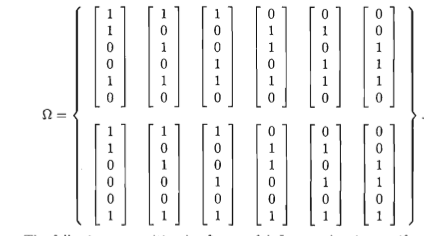
\includegraphics[height=1.2in]{omega.png}
			\label{fig:omega}
		\end{figure}		
	\end{itemize}	
\end{frame}

\begin{frame}[t]\frametitle{Example: Democratization Aid in the Republic of Georigia}
	\begin{itemize}
		\item<+-> The Republic of Georgia: recipient of US ``democratization aid'', foreign aid intended to bolster democratic processes. 
		\item<+-> Due to a previous history of fraudulent elections, US government and civil society groups wanted to encourage citizen monitoring of elections. 
		\item<+-> We conducted a program evaluation of one such
		effort: a simple information campaign to give voters the
		information necessary for filing a formal complaint with civil society
		groups or election officials if they witnessed problems on
		election day.
		\item<+->  The intervention consisted of sending canvassers to knock on
		doors and hand out fliers  in randomly selected precincts.
	\end{itemize}
\end{frame}

\begin{frame}[t]\frametitle{Example: Randomization Procedure}
	\begin{figure}[htbp]
		\centering
			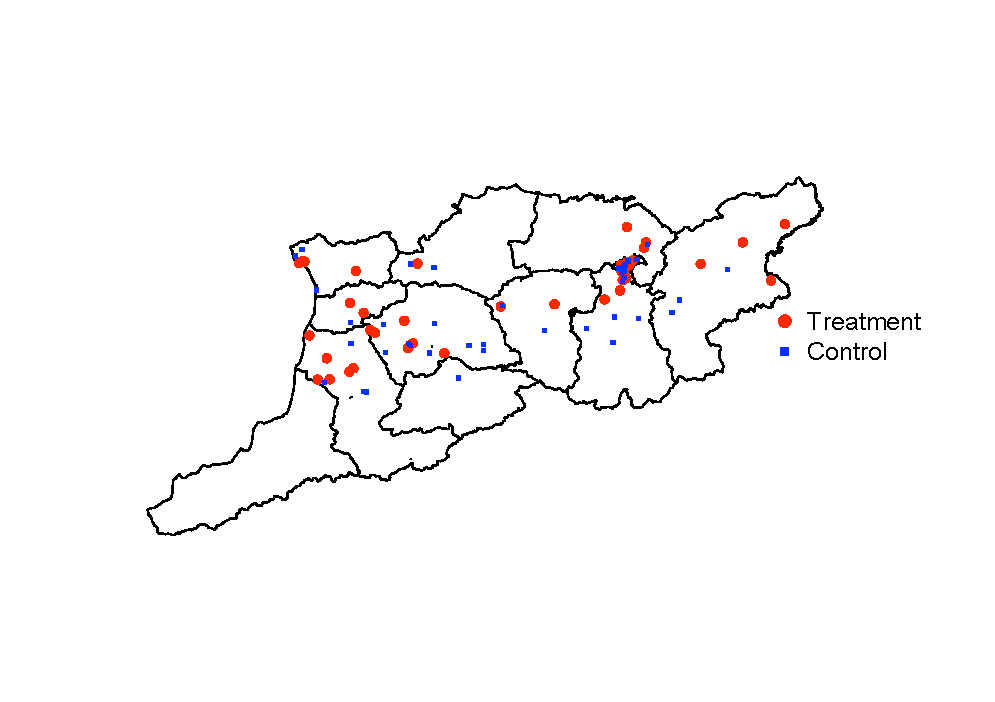
\includegraphics[height=1.7in]{experiment_map.pdf}
		\label{fig:experiment_map}
	\end{figure}
	Ths structure of randomization was as follows.
	\begin{itemize}
	\item 36 rural precincts were in blocks of 2, one treatment and one
	  control. So for these precincts, $m_s=1$ and $n_s = 2$.
	\item 48 urban precincts were in blocks of 4, two in treatment and and
	  two in control ($m_s=2$ and $n_s=4$). 
	\end{itemize}
\end{frame}

\begin{frame}[fragile]\frametitle{Some R code}
	How big is $\Omega$? 
		\begin{lstlisting}[frame=single]
		choose(2,1)^18 * choose(4,2)^12
		[1] 5.706304e+14
	\end{lstlisting}
	Let's create a function that will assign treatment repeatedly. 
	\begin{lstlisting}[frame=single]
		treat.assign <- function(treat,blocks=NA){
		  if(length(unique(blocks))==1){
		    treat.vector <- sample(treat)
		  }
		  else{
		  treat.vector <- tapply(treat,blocks,sample)
		  treat.vector <- unlist(treat.vector)
		  }
		  return(treat.vector)
		}
	\end{lstlisting}
	
\end{frame}

\begin{frame}[fragile]\frametitle{R Code}
	Let's create our distribution of treatment vectors. We could compute
	all $5.7 \times 10^{14}$ treatment vectors, but to save on computing
	time, we can sample a large number of possible treatment vectors to get
	``close-to-exact'' p-values. If our experiment were smaller, then 
	exhaustive enumeration would be better.
	
	Let's use the \texttt{replicate} function to  assign
	treatment 5,000 times and generate our $\Omega$:
	\begin{lstlisting}[frame=single]
	omega <- replicate(5000,
		              treat.assign(treat,blocks))
	omega <- unique(omega,MARGIN=2)
	\end{lstlisting}
	
\end{frame}

\section{The Null Hypothesis} % (fold)
\label{sec:sharp_null}
\begin{frame}[t]\frametitle{The Sharp Null}
	\begin{itemize}
		\item<+-> The most common hypothesis associated with randomization inference is
		the sharp null of no effect for all units. 
		\item<+->  A unit labeled as ``treated'' will have the exact same outcome as a unit
		labeled as ``control''. 
		\item<+->  Under the null, the  units' responses are \textit{fixed} and the only random element is the meaningless rotation of labels. 
		\item<+-> When testing the null hypothesis of no effect, the response of the
		\textit{i}th unit in stratum $s$ can be written $r_{si} $ and the
		vector of responses is $\textbf{r}$. 
	\end{itemize}	
\end{frame}

\section{Test Statistics} % (fold)
\label{sec:test_statistics}

% section test_statistics (end)
\begin{frame}[c]\frametitle{The Test Statistic}
	\begin{itemize}
		\item<+-> A \textbf{test statistic}
		$t(\mathbf{Z},r)$ is a quantity computed from the treatment assignment
		$\mathbf{Z}$ and the response $r$.
		\item<+-> The most commonly used test-statistic is the point estimate for the
		average treatment effect. In a block randomized experiment, the
		differences within blocks are summed, and each block difference is
		weighted by the proportion of units in the block:  
		$$ \sum_{s=1}^S
		\frac{n_s}{N}\sum_{i=1}^{n_s}\left\{\frac{Z_{si}r_{si}}{m_s}-\frac{(1-Z_{si})r_{si}}{n_s
		    - m_s}\right\}$$			
	\end{itemize}
\end{frame}

\begin{frame}[c]\frametitle{Significance Test}
	\begin{itemize}
		\item<+-> To compute the \emph{p}-value for any given test statistic, we
		simply calculate the proportion of treatment assignments
		$\textbf{z}$
		in $\Omega$ giving values of $t(\mathbf{z},\mathbf{r})$ greater
		than or equal to the observed $T$, namely:
		$$ \textrm{prob}\{t(\mathbf{Z},\mathbf{r} \geq T\} =
		\frac{| \{\mathbf{z} \in\Omega:t(\mathbf{z},\mathbf{r}) \geq T \}
		  |}{K}$$
		  \item<+-> The above p-value is for a one-tailed test. What about a two-tailed
		test?  There is some disagreement in the literature about this, but
		Rosenbaum recommends simply doubling the one-tailed p-value.
			\end{itemize}	
\end{frame}
\begin{frame}[c]\frametitle{Other Test Statistics}
	\begin{itemize}
		\item<+-> The default test-statistic is the difference in means, but many other
		are possible. 
		\item<+-> The difference in means test statistic will have low
		power in the presence of outliers, skewed distributions, or heavy
		tailed distributions. As a result, sometimes a more powerful test is
		desirable.
		\item<+->  One common alternative to the difference in means statistic is the \textbf{Wilcoxon
				\textit{rank sum} test}. In a completely randomized experiment, the
		responses are ranked from smallest to largest.
		\item<+-> If all $N$ responses
		were different numbers, the ranks woud be the numbers $1,2,...,N$.  If
		some of the responses were equal, then the average of their ranks
		would be used.
		\item<+-> Write $q_i$ for the rank of $r_i$, and write
		$\mathbf{q}=(q_i,...,q_N)^T$. The rank sum statistic is simply the sum
		of the ranks of the treated observations,
		i.e. $t(\mathbf{z},\mathbf{r})=\mathbf{Z^Tq}$. 
	\end{itemize}
\end{frame}

\begin{frame}[t]\frametitle{Rank Tests}
	\begin{itemize}
		\item<+-> \textbf{Stratified rank sum test}: For block randomized experiments, one easy extension of the rank sum test is to calculate the rank sum test separately in each strata and take the sum of these $S$ rank sums as the test statistic. 
		\item<+->\textbf{ Aligned rank test}: According to Hodges and Lehmann (1962), a more efficient rank test for block randomized experiment is the aligned rank statistic. For this statistic, subtract the mean of each stratum from the responses in that stratum, creating ``aligned responses'' . Rank the aligned responses without regard to block. The aligned rank statistic is the sum of the aligned ranks in the treated group.
		
	\end{itemize}
	
\end{frame}


\begin{frame}[t]\frametitle{Covariate Adjustment}
	\begin{itemize}
		\item<+-> Write $\tilde \epsilon(\cdot)$ for a function that creates residuals  ($\tilde \epsilon(\mathbf{r})=\mathbf{e}$)  from $\mathbf r$, which are the oucomes under the null hypothesis, and $\mathbf{X}$, which is a matrix of covariates.
		\item<+-> $\tilde \epsilon(\cdot)$ can be a simple linear model, some non-parametric
		smoother such as lowess, a robust linear model, etc.
		\item<+->  The point of adjustment is to reduce dispersion in $\mathbf{r}$, so choose  $\tilde \epsilon(\cdot)$  with that goal in mind.
		\item<+-> Remember that under the null hypothesis, nothing is stochastic except
		for the shuffling of treatment assignment labels. As a result
		$\mathbf{e}$ is a fixed quantity, not a random variable or a
		by-product of estimation.
		\item<+-> $\mathbf{e}$, however, may be less dispersed
		than $\mathbf{r}$ because some of the variation in $\mathbf{r}$ will
		have been captured by $\mathbf{X}$. 
	\end{itemize}	
\end{frame}

\begin{frame}[c]\frametitle{Covariate Adjustment}
	\begin{itemize}
		\item<+-> Under the null hypothesis, since $\mathbf{r_T}=\mathbf{r_c}$,
		$\mathbf{e_T}=\mathbf{e_C}$.
		\item<+-> So once can simply use the test
		statistic $t(\mathbf{z},\mathbf{e})$ instead of
		$t(\mathbf{z},\mathbf{r})$.
		\item<+-> With $\mathbf{e}$ in hand, just proceed as
		you would with $\mathbf{r}$.
	\end{itemize}
\end{frame}

\end{document}
